\section{Bayesian Statistics}
Bayesian statistics is based on \dfref{def:bayesian_statistics}, which follows the definition of subjective probability (\dfref{def:subjective_probability}) and the treating the parameters as realizations of a random variable (\axref{ax:parameter_variable}). The Bayesian framework originally come from the work of \citet{Bayes:63} and \citet{laplace_thorie_1812} with much of the modern discussions and formalism created later by \citet{Finetti1937LaP,Jeffreys1940} and \citet{Savage1954}.\newline
In the Bayesian paradigm, it is assumed that Natures decisions can be captured by a statistical model with parameters that are modeled as realizations of random variables. This means that the probability $p(S=s|X=x,D,I)$ in equation \EQref{eq:decision_rule3} depend on the parameters $w_1,\dots w_n$ of the statistical model. Introducing the shorthand notation $W=w_1\dots W=w_n \rightarrow w$, $dw_1\dots dw_n \rightarrow dw$ and $X=x \rightarrow x$, then
\begin{equation}
	\begin{split}
		p(s|x,D,I) &= \int dw p(w,s|x,D,I)\\
		& = \int dw p(s|w,x,D,I)p(w|x,D,I)
	\end{split}
	\label{eq:hest1}
\end{equation}
\begin{example}
	Writing out the shorthand notation
	\begin{equation}
		\begin{split}
			p(W=w_1,\dots,W= w_n,S = s|X = x,D,I)&\rightarrow p(w,s|x,D,I),\\
			dw_1\dots dw_n &\rightarrow dw.\\
		\end{split}
	\end{equation}
\end{example}

To evaluate $p(w|D,I)$ a combination of the chain rule (\thref{theorem:chain_rule}), Bayes' theorem (\thref{theorem:bayes_theorem}) and marginalization (\thref{theorem:law_of_total_probability}) can be employed viz
\begin{equation}
	\begin{split}
		p(w|x,D,I) &= p(w|D,I)\\
		&= \frac{p(D_s|w,D_x,I)p(w|I)}{p(D_s|D_x,I)},
	\end{split}
	\label{eq:pa2}
\end{equation}
where $D_s= \{s_i\}_{i=1}^n$, $D_x = \{x_i\}_{i=1}^n$ and $p(D_s|D_x,I)$ can be expanded via marginalization and \axref{ax:observation_relevance} has been used for the first and second equality.

\begin{axiom}[Relevance of Observations]
	\label{ax:observation_relevance}
	The Robot's observations are relevant for estimating Nature's model only when they map to known actions of Nature.
\end{axiom}

$p(w|I)$ is the Robot's prior belief about $w$. $p(D_s|w,D_x,I)$ is the likelihood of the past observations of Nature's actions, and $p(w|D,I)$ called the posterior distribution represent the belief of the Robot after seeing data. The prior distribution depends on parameters that must be specified and cannot be learned from data since it reflects the Robot's belief before observing data. These parameters are included in the background information, $I$. From \EQref{eq:pa2}, it is evident that, given the relevant probability distributions are specified, the probability of a parameter taking a specific value follows deductively from probability theory. The subjectivity arises from the assignment and specification of probability distributions which depend on the background information.



\subsection{Bayesian Regression}
\label{chp:regression}
Regression involves the Robot building a model, $f: \Omega_W\times \Omega_X\mapsto\mathbb{R}$, with associated parameters $w\in \Omega_W$, that estimates Nature's actions $S$ based on observed data $X$. Note that the output of $f$ is $\mathbb{R}$ implying that $S$ is assumed continuos. The model $f$ acts as a proxy for the Robot in that it on behalf of the Robot estimates the action of Nature given an input. Hence, in providing an estimate, the model must make a choice, similar to the Robot and thus the Robot must pick a cost function for the model. In this study, the quadratic cost function from \dfref{def:quadratic_cost} will be considered to review the subject. From \thref{theorem:expectation_decision_rule} the best action for the Robot can be written
\begin{equation}
	U^*(x,D) = \int ds s p(s|x,D,I)
	\label{eq:q1}
\end{equation}
Assuming the actions of Nature follow a normal distribution with the function $f$ as mean and an unknown precision, $\xi\in \Omega_W$
\begin{equation}
	p(s|x,w,\xi,I)=\sqrt{\frac{\xi}{2\pi}} e^{-\frac{\xi}{2}(f(w,x)-s)^2}.
	\label{f_dist}
\end{equation}
Using \EQref{f_dist} and marginalizing over $\xi,w$
\begin{equation}
	\begin{split}
		p(s|x,D,I) &= \int p(s,w,\xi|x,D,I) dw d\xi\\
		& = \int p(s|x,w,\xi,D,I)  p(w,\xi|x,D,I)dw d\xi\\
		& = \int p(s|x,w,\xi,I)  p(w,\xi|D,I)dw d\xi,\\
	\end{split}
	\label{eq:q2}
\end{equation}
where it has been used that $p(s|w,\xi,x,D,I) = p(s|w,\xi,x,I)$ since by definition $f$ produce a $1-1$ map of the input $x$ (\EQref{f_dist}) and $p(w,\xi|x,D,I) = p(w,\xi|D,I)$ from \axref{ax:observation_relevance}. Using \EQref{eq:q2} in \EQref{eq:q1}\footnote{Note that a function of a random variable is itself a random variable, so $f$ is a random variable.}
\begin{equation}
	\begin{split}
		U^*(x,D) & = \int f(w,x)  p(w,\xi|D,I) dw d\xi,\\
		& = \mathbb{E}[f|x,D,I]
	\end{split}
	\label{eq:q3}
\end{equation}	
where it has been used that
\begin{equation}
	\begin{split}
		\mathbb{E}[S|x,w,\xi,I] &= \int s p(s|x,w,\xi,I) ds\\
		&= f(w,x)
	\end{split}
\end{equation}
according to \EQref{f_dist}. Using Bayes theorem (\thref{theorem:bayes_theorem})
\begin{equation}
	p(w,\xi|D,I) = \frac{p(D_s|D_x,w,\xi,I)p(w,\xi|D_x,I)}{p(D_s|D_x,I)}
	\label{eq:bayes2}
\end{equation}
where from marginalization (\thref{theorem:law_of_total_probability})
\begin{equation}
	p(D_s|D_x,I) = \int p(D_s|D_x,w,\xi,I)p(w,\xi|D_x,I) dw d\xi.
\end{equation}
Assuming the past actions of Nature are independent and identically distributed, the likelihood can be written (using equation \EQref{f_dist})
\begin{equation}
	p(D_s|D_x,w,\xi,I) = \bigg(\frac{\xi}{2\pi}\bigg)^\frac{n}{2}\prod_{i=1}^n e^{-\frac{\xi}{2}(f(w,x_i)-s_i)^2}
	\label{reg:likelihood}
\end{equation}
From the chain rule (see \thref{theorem:chain_rule}) and \thref{ax:observation_relevance}
\begin{equation}
	p(w,\xi|D_x,I) = p(w|\xi,I)p(\xi|I).
\end{equation}
Assuming the distributions of the $w$'s are i) independent of $\xi$ and ii) normally distributed\footnote{The normally distributed prior is closely related to weight decay~\citep{Plaut1986}, a principle conventionally used in frequentist statistics to avoid the issue of overfitting.} with zero mean and a precision described by a hyperparameter, $\lambda$. 	 
\begin{equation}
	\begin{split}
		p(w|\xi,I) & = p(w|I)\\
		& = \int p(w|\lambda,I)p(\lambda|I)d\lambda
	\end{split}
	\label{eq:prior1}
\end{equation}
The precision is constructed as a wide gamma distribution\index{Gamma distribution} so as to approximate an objective prior
\begin{equation}
	p(w|\lambda,I)p(\lambda|I)
	= \prod_{q=1}^{\tilde{n}} \frac{\lambda_q^\frac{n_q}{2}}{(2\pi)^\frac{n_q}{2}}e^{-\frac{\lambda_q}{2}\sum_{l=1}^{n_q}w_l^2}\frac{\beta_q^{\alpha_q}}{\Gamma(\alpha_q)}\lambda_q^{\alpha_q-1}e^{-\beta_q \lambda_q}
	\label{eq:prior}
\end{equation}
where $\alpha_q,\beta_q$ are prior parameters (a part of the background information) and $\tilde{n}$ is the number of hyper parameters. In the completely general case $\tilde{n}$ would equal the number of parameters $w$, such that each parameter has an independent precision. In practice, the Robot may consider assigning some parameters the same precision, e.g. for parameters in the same layer in a neural network. Since $p(\xi|I)$ is analogous to $p(\lambda|I)$ -- in that both are prior distributions for precision parameters -- $p(\xi|I)$ is assumed to be a wide gamma distribution, then
\begin{equation}
	\begin{split}
		p(\xi|I) & = \text{Ga}(\xi|\tilde{\alpha},\tilde{\beta})\\
		& =\frac{\tilde{\beta}^{\tilde{\alpha}}}{\Gamma(\tilde{\alpha})}\xi^{\tilde{\alpha}-1}e^{-\tilde{\beta} \xi}.
	\end{split}
	\label{p7}
\end{equation}
At this point equation \EQref{eq:q1} is fully specified (the parameters $\alpha,\beta,\tilde{\alpha},\tilde{\beta}$ and the functional form of $f(w,x)$ are assumed specified as part of the background information) and can be approximated by obtaining samples from $p(w,\xi,\lambda|D,I)$ via HMC~\citep{Hammersley1964,Duane:1987de,Neal:1996,Neal2012} (see \appref{app:HMC} for a review of HMC). The centerpiece in the HMC algorithm is the Hamiltonian defined viz~\citep{Neal:1996,Neal2012}
\begin{equation}
	H \equiv  \sum_{q=1}^{\tilde{n}}\sum_{l=1}^{n_q}\frac{p_{l}^2}{2m_{l}}-\ln[p(w,\xi,\lambda|D,I)]+const,
	\label{eqh}
\end{equation}
where 
\begin{equation}
	p(w,\xi|D,I) = \int d\lambda p(w,\xi,\lambda|D,I).
	\label{eq:ss}
\end{equation}
Besides its function in the HMC algorithm, the Hamiltonian represent the details of the Bayesian model well and should be a familiar sight for people used to the more commonly applied frequentist formalism\index{Frequentist statistics} (since, in this case, it is in form similar to a cost function comprised of a sum of squared errors, weight decay on the coefficients and further penalty terms~\citep{hastie_09,murphy2013machine,Goodfellow2016}). Using \EQref{eq:bayes2}-\EQref{eq:ss} yields
\begin{equation}
	\begin{split}
		H&=\sum_{q=1}^{\tilde{n}}\sum_{l=1}^{n_q}\frac{p_{l}^2}{2m_{l}}+\frac{n}{2}[\ln(2\pi)-\ln(\xi)] +\frac{\xi}{2}\sum_{i=1}^{n}(f(w,x_i)-s_i)^2\\
		&\quad+\sum_{q=1}^{\tilde{n}}\bigg(\ln(\Gamma(\alpha_q))-\alpha_q\ln(\beta_q)+(1-\alpha_q)\ln(\lambda_q)+\beta_q\lambda_q\\
		&\qquad\qquad+\frac{n_q}{2}(\ln(2\pi)-\ln(\lambda_q))+\frac{\lambda_q}{2}\sum_{l=1}^{n_q}w_l^2\bigg)\\
		&\quad+\ln(\Gamma(\tilde{\alpha}))-\tilde{\alpha}\ln(\tilde{\beta})+(1-\tilde{\alpha})\ln(\xi)+\tilde{\beta}\xi+const.
	\end{split}
	\label{eqh2}
\end{equation}
\begin{example}
	\index{Example: HMC Hamiltonian variable change}
	Let $\xi \equiv e^\zeta$, such that $\zeta\in [-\infty,\infty]$ maps to $\xi\in[0,\infty]$ and $\xi$ is ensured to be positive definite regardless of the value of $\zeta$. Using the differential $d\xi =  \xi d\zeta$ in \EQref{eq:q3} means $p(\theta,\xi,\lambda|D,I)$ is multiplied with $\xi$. Hence, when taking $-\ln(p(\theta,\xi,\lambda|D,I))$ according to \EQref{eqh}, a $-\ln(\xi)$ is added to the Hamiltonian. In practice this means
	\begin{equation}
		(1-\tilde{\alpha})\ln(\xi)\in H\Rightarrow -\tilde{\alpha}\ln(\xi).
	\end{equation} 	
\end{example}



\begin{example}
	Suppose there is a game between a Robot and Nature in which the Robot objective is to guess the position of the Robot. The Robot is given measurements of its velocity and acceleration, at any time step and must formulate a belief about its position. Nature decides the true position of the Robot and will penalize the Robot according to the deviation between the Robots estimate of its position and the true position viz (\dfref{def:quadratic_cost})
	\begin{equation}
		C(U(x),s) = (U(x)-s)^2,
	\end{equation}
	where $s$ is the true position $U(x)$ is the Robots estimate based on data $x$ containing velocity and acceleration measurements. 
	\begin{figure}[H]
		\centering
		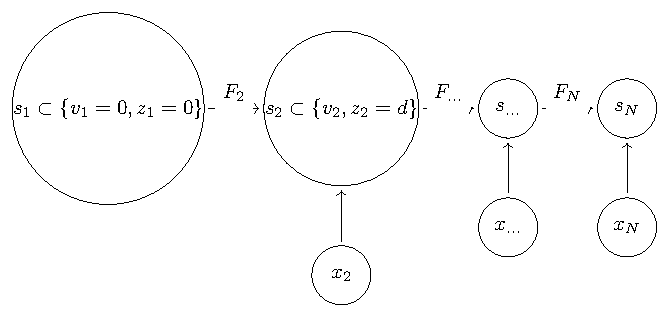
\includegraphics[width = 0.8\textwidth]{figures/graph.pdf}
		\caption{}
		\label{fig:1}
	\end{figure}
	Suppose the Robot is given all historical data, then the expected cost can be written
	\begin{equation}
		\mathbb{E}_{S|X}[C(U(X),S|s_1,\{x\}_{2:N},I)] = \int ds (U(x_N)-s)^2p(s|s_1,\{x\}_{2:N},I).
	\end{equation}
	The optimal decision is defined by
	\begin{equation}
		\frac{d}{dU(X)}\bigg(\mathbb{E}_{S|X}[C(U(X),S|s_1,\{x\}_{2:N},I)]\bigg)\bigg|_{U(x_N)=U^*(x_N)} = 0
	\end{equation}
	leading to (\thref{theorem:expectation_decision_rule})
	\begin{equation}
		U^*(x_N) = \mathbb{E}[S_{N}|s_1,\{x\}_{2:N},I].
		\label{eq:dr}
	\end{equation}
	The inutitive interpretation of \EQref{eq:dr} is that the optimal decision of the Robot is to estimate the position that it expects Nature to have chosen. Now
	\begin{equation}
		\mathbb{E}[S_{N}|s_1,\{x\}_{2:N},I] = \int ds_{N} s_N p(s_N|s_1,\{x\}_{2:N},I).
		\label{eq:a5}
	\end{equation}
	Assume that
	\begin{equation}
		\begin{split}
			p(s_i|s_{i-1},I) &= N(s_i|\mu_i = F_is_{i-1}+b_i,\Sigma_i = Q_i),\\
			p(x_i|s_{i},I) &= N(x_i|\mu_i = H_is_{i}+d_i,\Sigma_i = R_i)
		\end{split}
		\label{eq:a2}
	\end{equation}
	Hence, $p(s_N|s_1,\{x\}_{2:N},I)$ must be reformulated such that the above can be utilized. 
	Now
	\begin{equation}
		\begin{split}
			p(s_N|s_1,\{x\}_{2:N},I) &= \frac{p(x_{N}|s_N,s_1,\{x\}_{2:N-1},I)p(s_N|s_1,\{x\}_{2:N-1},I)}{p(x_{N}|s_1,\{x\}_{2:N-1},I)}\\
			&= \frac{p(x_{N}|s_N,I)p(s_N|s_1,\{x\}_{2:N-1},I)}{p(x_{N}|s_1,\{x\}_{2:N-1},I)}\\
		\end{split}
		\label{eq:a3}
	\end{equation}
	where
	\begin{equation}
		\begin{split}
			p(s_N|s_1,\{x\}_{2:N-1},I) &= \int ds_{N-1}p(s_N,s_{N-1}|s_1,\{x\}_{2:N-1},I)\\
			&= \int ds_{N-1}p(s_N|s_{N-1})p(s_{N-1}|s_1,\{x\}_{2:N-1},I)\\
			&=N(s_{N}|\mu_{N|N-1},\Sigma_{N|N-1})
		\end{split}
		\label{eq:a1}
	\end{equation}
	where 
	\begin{equation}
		\begin{split}
			\mu_{N|N-1} &= F_{N}\mu_{N-1}+b_N\\
			\Sigma_{N|N-1} &= F_{N}\Sigma_{N-1}F_{N}^T+Q_{N}\\
		\end{split}
	\end{equation}
	Using \EQref{eq:a1} and \EQref{eq:a2} in \EQref{eq:a3} then yields~\citep{murphy2023probabilistic}
	\begin{equation}
		p(s_N|s_1,\{x\}_{2:N},I) = N(s_N|\mu_{N},\Sigma_N)
		\label{eq:a4}
	\end{equation}
	where
	\begin{equation}
		\begin{split}
			\mu_{N} &= \mu_{N|N-1}+K_N(x_N-\hat{x}_N),\\
			\Sigma_{N} &= \Sigma_{N|N-1}-K_NS_NK_N^T,\\
			K_N & = \Sigma_{N|N-1}H_N^TS_N^{-1},\\
			\hat{x}_N&= H_N\mu_{N|N-1}+d_N,\\
			S_N & = H_N\Sigma_{N|N-1}H_N^T+R_N\\
		\end{split}
	\end{equation}
	Combining \EQref{eq:a4} with \EQref{eq:a5} then yields the optimal decision for the Robot
	\begin{equation}
		\mathbb{E}[S_{N}|s_1,\{x\}_{2:N},I] = \mu_{N}.
	\end{equation}
	
\end{example}

\begin{example}
	Consider a Robot moving in one dimension. Every time interval $\Delta t$, the Robot will sample a wheel counter and an accelerometer. The wheel counter will be incremented every distance $d$. The Robot is interested in knowing its position and velocity. Expand the position viz
	\begin{equation}
		z(t+\Delta t)=z(t)+\Delta t \frac{dz(t)}{dt}+\frac{1}{2}(\Delta t)^2\frac{d^2z(t)}{dt^2}+\mathcal{O}(\Delta t^3)
	\end{equation}
	which discretize to
	\begin{equation}
		z_k\simeq z_{k-1}+\Delta t v_{k-1}+\frac{1}{2}(\Delta t)^2a_{k-1},
	\end{equation}
	where $\Delta t = \text{const}$ and
	\begin{equation}
		\begin{split}
			v_k &\simeq v_{k-1}+\Delta t a_{k-1},\\
			a_k &\simeq a_{k-1},
		\end{split}
	\end{equation}
	This means
	\begin{equation}
		\begin{split}
			s_k &= \begin{pmatrix}
				z_k\\ v_{k} \\ a_k\\
			\end{pmatrix}\\
			& \simeq \underbrace{\begin{pmatrix}
					1 & \Delta t & \frac{1}{2}\Delta t^2  \\
					0 & 1 & \Delta t  \\
					0 & 0 & 1  \\
			\end{pmatrix}}_{=F_k}\begin{pmatrix}
				z_{k-1}\\ v_{k-1} \\ a_{k-1}\\
			\end{pmatrix}
		\end{split}
	\end{equation}
	where $b_k=\emptyset$ for simplicity. Now take
	\begin{equation}
		\begin{split}
			x_k &= \begin{pmatrix}
				c_k \\ a_k
			\end{pmatrix}\\
			&= \underbrace{\begin{pmatrix}
					d^{-1} & 0 & 0\\
					0 & 0 & 1 
			\end{pmatrix}}_{=H_k}\begin{pmatrix}
				z_{k-1}\\ v_{k-1} \\ a_{k-1}\\
			\end{pmatrix}+r_k
		\end{split}
	\end{equation}
	where $r_k \sim N(0,R_k)$ with 
	\begin{equation}
		R_k = \begin{pmatrix}
			\sigma_z^2 & \sigma_z\sigma_a\\
			\sigma_z\sigma_a & \sigma_a^2 \\
		\end{pmatrix},
	\end{equation}
	where $\sigma_z$ and $\sigma_a$ are estimated from observations. The process noise can be determined viz~\href{https://github.com/rlabbe/Kalman-and-Bayesian-Filters-in-Python/blob/master/07-Kalman-Filter-Math.ipynb}{Kalman link}
	\begin{equation}
		Q_k = \begin{pmatrix}
			\frac{\Delta t^4}{4} & \frac{\Delta t^3}{2} & \frac{\Delta t^2}{2}\\
			\frac{\Delta t^3}{2} & \Delta t^2 & \Delta t\\
			\frac{\Delta t^2}{2} & \Delta t & 1\\
		\end{pmatrix}\sigma^2,
	\end{equation}
	where $\sigma \sim \Delta a$.
\end{example}


\subsection{Bayesian Classification}
\label{chp:baycl}
Classification is the discrete version of regression, meaning it involves the Robot building a model,\begin{equation}
	f: \Omega_W \times \Omega_X \mapsto \Delta^K, \quad w \in \Omega_W,
\end{equation}
where $\Delta^K$ is the $K$-dimensional probability simplex and $\Omega_S = \{1,\dots,K\}$ represents Nature's discrete action (class label). As opposed to regression, the random variable $S$ is now discrete and the function is identified with the probability of each action
\begin{equation}
	p(S = s|x,w,I)= f_{S = s}(w,x),
	\label{f_dist2}
\end{equation}
with
\begin{equation}
	\sum_{s\in \Omega_S} p(S = s|x,w,I) = 1.
\end{equation}
In this case, the Robot's action space is equal to Natures action space, with the possible addition of a reject option, $\Omega_U=\Omega_S\cup \text{"Reject"}$. To review this subject the Robot will be considered to be penalized equally in case of a classification error, which corresponds to the $0-1$ cost function, with the addition of a reject option at cost $\lambda$. This means
\begin{equation}
	C(U(\tilde{D}),s) = 1- \delta_{U(\tilde{D}),s}+(\lambda-1)\delta_{U(\tilde{D}),\text{"Reject"}}.
\end{equation}
The optimal decision rule for the robot can the be written (\EQref{eq:conditional_cost_discrete})
\begin{equation}
	\begin{split}
		U^*(\tilde{D}) & = \arg\min_{U(\tilde{D})}\mathbb{E}_{S|\tilde{D}}[C(U(\tilde{D}), S)|\tilde{D},I]\\
		&= \arg\min_{U(\tilde{D})}\bigg(\sum_{s\in \Omega_S}C(U(\tilde{D}),s)p(S = s|\tilde{D},I)+(\lambda-1)\delta_{U(\tilde{D}),\text{"Reject"}}\bigg)\\
		& = \arg\min_{U(\tilde{D})}\bigg(1- p(S=U(\tilde{D})|\tilde{D},I)+(\lambda-1)\delta_{U(\tilde{D}),\text{"Reject"}}\bigg).
	\end{split}
	\label{eq:expected_cost1}
\end{equation}
In absence of the reject option, the optimal decision rule is to pick the MAP, similar to \thref{theorem:MAP}. Using \EQref{f_dist2} and marginalizing over $w$
\begin{equation}
	\begin{split}
		p(S= U(\tilde{D})|\tilde{D},I) &= \int p(S = U(\tilde{D}),w|\tilde{D},I) dw \\
		& = \int p(S = U(\tilde{D})|w,\tilde{D},I)  p(w|\tilde{D},I)dw \\
		& = \int p(S = U(\tilde{D})|x,w,I)  p(w|D,I)dw \\
		& = \int f_{S = U(\tilde{D})}(w,x)  p(w|D,I)dw \\
		& = \mathbb{E}[f_{S = U(\tilde{D})}(w,x)|D,I],\\
	\end{split}
	\label{eq:q5}
\end{equation}
where for the second to last equality it has been assumed that
\begin{equation}
	p(S = U(\tilde{D})|w,\tilde{D},I) = p(S = U(\tilde{D})|w,x,I)
\end{equation}
since by definition $f$ (see \EQref{f_dist2}) produce a $1-1$ map of the input $x$ and $p(w|\tilde{D},I) = p(w|D,I)$ from \axref{ax:observation_relevance}. From Bayes theorem
\begin{equation}
	p(w|D,I) =\frac{p(D_s|D_x,w,I)p(w|D_x,I)}{p(D_s|D_x,I)},
\end{equation}
where from \axref{ax:observation_relevance} $p(w|D_x,I) = p(w|I)$. Assuming the distribution over $w$ is normally distributed with zero mean and a precision described by a hyperparameter, $\lambda$, 
\begin{equation}
	p(w|I) = \int p(w|\lambda,I)p(\lambda|I)d\lambda.
\end{equation}
where $p(w|\lambda,I)p(\lambda|I)$ is given by \EQref{eq:prior}. Assuming the past actions of Nature are independent and identically distributed, the likelihood can be written~\citep{Fischer1999} 
\begin{equation}
	\begin{split}
		p(D_s|D_x,w,I) &=\prod_{i=1}^{n}p(S = s_i|X = x_i,w,I)\\
		&=\prod_{i=1}^{n}f_{S = s_i}(w,x_i)\\
	\end{split}.
	\label{lik}
\end{equation}
At this point \EQref{eq:expected_cost1} is fully specified and can be approximated by HMC similarly to the regression case. In this case, the model can be represented by the Hamiltonian 
\begin{equation}
	H \equiv  \sum_{q}\sum_{l}\frac{p_{l}^2}{2m_{l}}-\ln(p(w,\lambda|D,I))+const
	\label{ham3}
\end{equation}
where
\begin{equation}
	p(w|D,I) = \int d\lambda p(w,\lambda|D,I).
\end{equation}
Using \EQref{eq:q5}-\EQref{lik} in equation \eqref{ham3} yields the Hamiltonian
\begin{equation}
	\begin{split}
		H&=\sum_{q=1}^{\tilde{n}}\sum_{l=1}^{n_q}\frac{p_{l}^2}{2m_{l}}-\sum_{i=1}^{n}\ln(f_{S = s_i}(w,x_i))+\text{const}\\
		&\quad+\sum_{q=1}^{\tilde{n}}\bigg(\ln(\Gamma(\alpha_q))-\alpha_q\ln(\beta_q)+(1-\alpha_q)\ln(\lambda_q)+\beta_q\lambda_q\\
		&\qquad \qquad+\frac{n_q}{2}(\ln(2\pi)-\ln(\lambda_q))+\frac{\lambda_q}{2}\sum_{l=1}^{n_q}w_l^2\bigg)\\
	\end{split}.
	\label{ham2}
\end{equation}
Sampling \EQref{ham2} yields a set of coefficients which can be used to compute $\mathbb{E}[f_s(w,x)|D,I]$ which in turn (see \EQref{eq:expected_cost1}) can be used to compute $U^*(\tilde{D})$.


\subsection{Making Inference About the Model of Nature}
In some instances, the robot is interested in inference related to the model of Nature. The observation $X=x$ by definition does not have an associated known action of Nature and thus by \axref{ax:observation_relevance} is disregarded in this context. From \EQref{eq:decision_rule3}
\begin{equation}
	U^*(D) = \arg\min_{U(D)} \mathbb{E}_{S|D}[C(U(D), S)|D,I]
	\label{eq:best_decision}
\end{equation}
where $S=s$ is interpreted as an action related to the model of Nature, e.g. Nature picking a given systematic that generates data.


\subsubsection{Selecting the Robot's Model}
\label{sec:model_selection}
Suppose the Robot must choose between two competing models, aiming to select the one that best represents Nature's true model. The two competing models could e.g. be two different functions $f$ in regression or two different probability distribution assignments. In this case the Robot has actions $u_1$ and $u_2$ representing picking either model and Nature has two actions $s_1$ and $s_2$ which represent which model that in truth fit Nature's true model best. From \EQref{eq:best_decision}
\begin{equation}
	\begin{split}
		\mathbb{E}[C(u_1, S)|D,I] =&  \sum_{s = s_1,s_2}C(u_1,s)p(S=s|D,I),\\
		\mathbb{E}[C(u_2, S)|D,I] =&  \sum_{s = s_1,s_2}C(u_2,s)p(S=s|D,I),
	\end{split}
\end{equation}
where in this case $u_i=s_i\quad \forall (u_i,s_i)\in \Omega_U\times\Omega_S$ but the notational distinction is kept to avoid confusion. Since there is no input $X=x$ in this case, the decision rule $U$ is fixed (i.e. it does not depend on $x$). $U = u_1$ is picked iff $\mathbb{E}[C(U = u_1, S)|D,I]<\mathbb{E}[C(U = u_2, S)|D,I]$, meaning
\begin{equation}
	\frac{p(s_1|D,I)}{p(s_2|D,I)}>\frac{C(u_1,s_2)-C(u_2,s_2)}{C(u_2,s_1)-C(u_1,s_1)}.
\end{equation}
The ratio $\frac{p(s_1|D,I)}{p(s_2|D,I)}$ is referred to as the posterior ratio\index{Posterior ratio}. Using Bayes theorem it can be re-written viz
\begin{equation}
	\begin{split}
		\text{posterior ratio} &= \frac{p(s_1|D,I)}{p(s_2|D,I)}\\
		& = \frac{p(D_s|s_1,D_x,I)p(s_1|I)}{p(D_s|s_2,D_x,I)p(s_2|I)},
	\end{split}
\end{equation}
where for the second equality it has been used that the normalization $p(D|I)$ cancels out between the denominator and nominator and \axref{ax:observation_relevance} has been employed. Given there is no a priori bias towards any model, $p(s_1|I) = p(s_2|I)$
\begin{equation}
	\text{posterior ratio} = \frac{p(D_s|s_1,D_x,I)}{p(D_s|s_2,D_x,I)}.
	\label{eq:bayes_factor}
\end{equation}
$p(D_s|s_1,D_x,I)$ and $p(D_s|s_2,D_x,I)$ can then be expanded via marginalization, the chain rule and Bayes theorem until they can be evaluated either analytically or numerically. \EQref{eq:bayes_factor} is referred to as Bayes factor\index{Bayes factor} and as a rule of thumb

\begin{definition}[Bayes Factor Interpretation Rule of Thumb]
	If the probability of either of two models being the model of Nature is more than 3 times likely than the other, the likelier model is accepted. Otherwise the result does not significantly favor either model.
\end{definition}

\subsubsection{Bayesian Parameter Estimation}
Let $w\in \Omega_W$ represent a parameter with the associated random variable $W$. In case of parameter estimation, the action of Nature is identified with the parameter of interest from the model of Nature's and the Robot's action with the act of estimating the parameters value, meaning (\EQref{eq:decision_rule3})
\begin{equation}
	U^*(D)=\arg\min_{U(D)}\mathbb{E}_{W|D}[C(U(D), W)|D,I],
\end{equation}
with
\begin{equation}
	\mathbb{E}_{W|D}[C(U(D), W)|D,I] = \int dw C(U(D),w)p(w|D,I).
\end{equation}
At this point, the Robot can select a cost function like in \secref{sec:assing_cost} and proceed by expanding $p(w|D,I)$ similarly to \EQref{eq:pa2}. Picking the quadratic cost (\dfref{def:quadratic_cost}) yields 
\begin{equation}
	\begin{split}
		U^*(D) = \mathbb{E}_{W|D}[W|D,I]
	\end{split}
	\label{eq:hest2}
\end{equation}
$p(w|D,I)$ in \EQref{eq:hest2} can be expanded as shown in \EQref{eq:pa2}.

\begin{example}
	Consider the scenario where two sets of costumers are subjected to two different products, $A$ and $B$. After exposure to the product, the costumer will be asked whether or not they are satisfied and they will be able to answer "yes" or "no" to this. Denote the probability of a costumer liking product $A/B$ by $w_A/w_B$, respectively. In this context, the probabilities $w_A/w_B$ are parameters of Natures model (similar to how the probability is a parameters for a binomial distribution). What will be of interest is the integral of the joint probability distribution where $w_B>w_A$, meaning
	\begin{equation}
		p(w_B > w_A|D,I)= \int_0^1\int_{w_A}^1p(w_A,w_B|D,I)dw_Adw_B.
		\label{e1}
	\end{equation}
	Assuming the costumer sets are independent
	\begin{equation}
		\begin{split}
			p(w_A,w_B|D,I) &= p(w_B|w_A,D,I)p(w_A|D,I)\\
			& = p(w_B|D_A,I)p(w_A|D_A,I),
		\end{split}
	\end{equation}
	with
	\begin{equation}
		p(w_i|D_i,I)=\frac{p(D_i|w_i,I)p(w_i|I)}{p(D_i|I)}.
	\end{equation}
	Assuming a beta prior and a binomial likelihood yields (since the binomial and beta distributions are conjugate)
	\begin{equation}
		p(w_i|D_i,I)=\frac{w_i^{\alpha_i-1}(1-w_i)^{\beta_i-1}}{B(\alpha_i,\beta_i)},
	\end{equation}
	where $\alpha_i\equiv \alpha+s_i$, $\beta_i\equiv \beta+f_i$ and $s_i/f_i$ denotes the successes/failure, respectively, registered in the two sets of costumers. Evaluating \EQref{e1} yields
	\begin{equation}
		p(w_B > w_A|D,I)= \sum_{j=0}^{\alpha_B-1}\frac{B(\alpha_A+j,\beta_A+\beta_B)}{(\beta_B+j)B(1+j,\beta_B)B(\alpha_A,\beta_A)}.
	\end{equation}
	
\end{example}



